% !TeX root = ../beamer.tex
\section{Signal Korrelation}

\begin{frame}
    \frametitle{Ermittlung der bistatischen Entfernung}

    \begin{itemize}
        \centering
        \item Bestimmung der \textbf{bistatischen Entfernung} aus gemessenem \textbf{Zeitversatz} \(\tau\) zwischen \textbf{Echo-} und \textbf{Referenzsignal}:
              \begin{equation}
                  R = \tau \tikzmarknode{c}{c}
              \end{equation}
              \tikzmarknode{c_txt}{Lichtgeschwindigkeit \(\approx\) \SI[per-mode=symbol]{3e8}{\metre\per\second}}
              \begin{tikzpicture}[remember picture,overlay]
                  \draw [->] (c_txt) to [bend right,in=-100,out=90] (c.south);
              \end{tikzpicture}

              \vspace{\baselineskip}

        \item<2-> \textbf{Wie wird Zeitversatz \(\tau\) gemessen?}
    \end{itemize}
\end{frame}

\begin{frame}
    \frametitle{Referenz- und Echosignal}

    Gepulstes Beispiel:
    \begin{columns}
        \begin{column}{0.5\textwidth}
            \begin{figure}
                \centering
                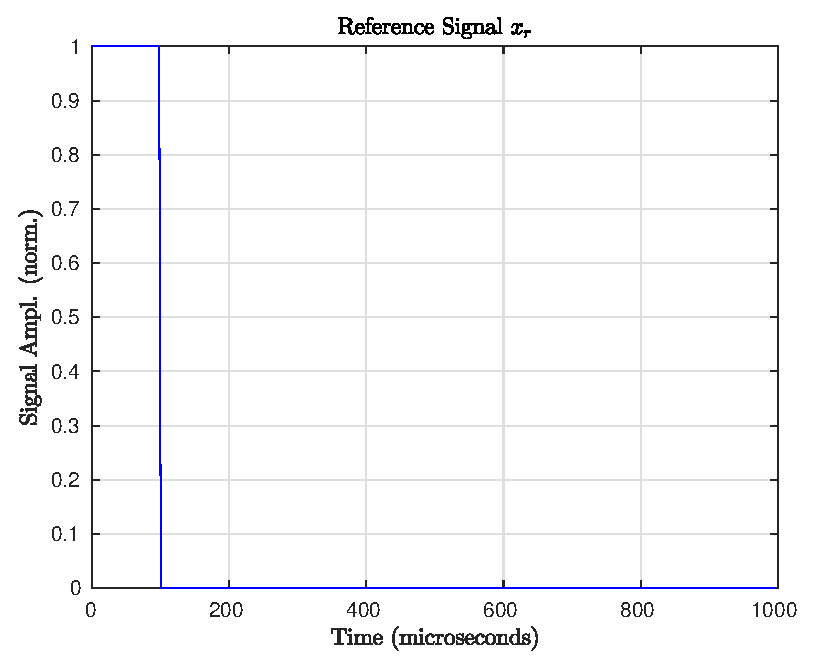
\includegraphics[width=\linewidth,height=\textheight-5\baselineskip,keepaspectratio]{reference_signal.eps}
            \end{figure}
        \end{column}
        \begin{column}{0.5\textwidth}
            \begin{figure}
                \centering
                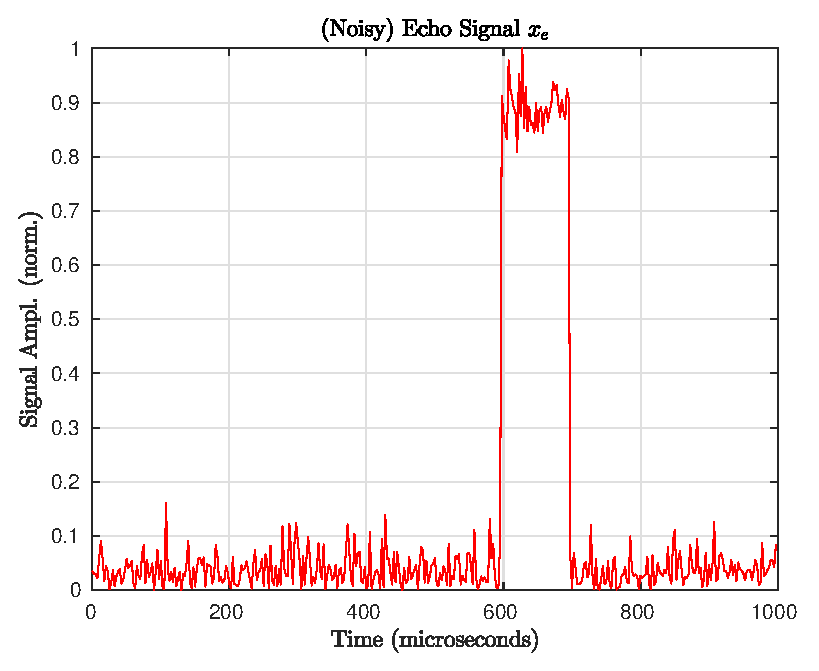
\includegraphics[width=\linewidth,height=\textheight-5\baselineskip,keepaspectratio]{echo_signal.eps}
            \end{figure}
        \end{column}
    \end{columns}
\end{frame}

\begin{frame}
    \frametitle{Kreuzkorrelation}

    \begin{figure}
        \centering
        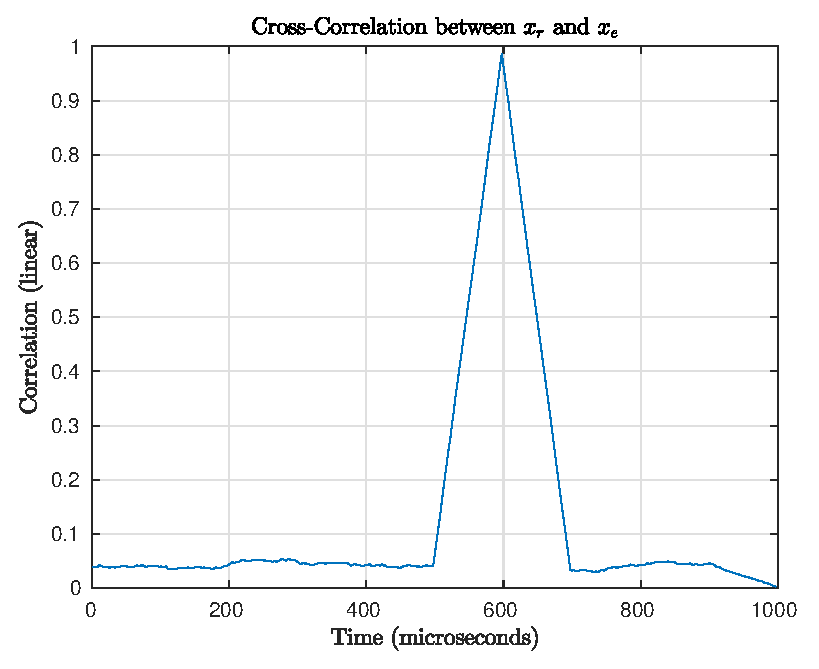
\includegraphics[width=\linewidth,height=\textheight-3\baselineskip,keepaspectratio]{correlation_linear.eps}
    \end{figure}
\end{frame}

\begin{frame}
    \frametitle{Range-Doppler Map}

    \begin{figure}
        \centering
        \includegraphics[width=\linewidth,height=\textheight-5\baselineskip,keepaspectratio]{range_doppler.png}
        \caption{Ausschnitt aus Kreuzambiguitätsfunktion für bewegtes Ziel~\cite[p.~161]{Malanowski2019}.}
    \end{figure}
\end{frame}

\begin{frame}
    \frametitle{Transformation in Kartesische Koordinaten}

    \Large Wie gelangt man von \textbf{bistatischer} zur \textbf{kartesischen Darstellung}?\normalsize

    \vspace{2\baselineskip}

    Möglichkeiten:
    \begin{enumerate}
        \item \textbf{Antennenrichtwirkung} nutzen um bistatischen Ellipsoiden \emph{abzutasten}
        \item \textbf{Ellipsoiden} verschiedener Rx-Tx Paare \textbf{übereinanderlegen}
    \end{enumerate}
\end{frame}

\begin{frame}
    \frametitle{Schnittpunkte der bistatischen Ellipse}

    \begin{figure}
        \centering
        \begin{adjustbox}{max width=\linewidth,totalheight=\textheight-5\baselineskip}
            \begin{tikzpicture}
                
\coordinate (rx1_coord) at (-5,0);
\coordinate (tx1_coord) at (5,0);
\coordinate (tx2_coord) at (2,2);
\coordinate (tx3_coord) at (6,-3);
\coordinate (target_coord) at (-2,-3.5);

\draw [visible on=<2->,red]
let
\p1=(tx1_coord),
\p2=($(target_coord)-(\p1)$),
\p3=($(target_coord)-(rx1_coord)$),
\p4=($(\p1)-(rx1_coord)$),
\n1={scalar((veclen(\x2,\y2) + veclen(\x3,\y3))*1pt/1cm)},
\n2={scalar(veclen(\x4,\y4)*1pt/1cm)},
\n3={sqrt(pow(\n1/2, 2))},
\n4={sqrt(pow(\n1/2, 2) - pow(\n2/2, 2))},
in
($(rx1_coord)!0.5!(\p1)$)
circle [x radius=\n3,y radius=\n4,draw=gray];

\draw [visible on=<3->,green]
let
\p1=(tx2_coord),
\p2=($(target_coord)-(\p1)$),
\p3=($(target_coord)-(rx1_coord)$),
\p4=($(\p1)-(rx1_coord)$),
\p5=(rx1_coord),
\n1={scalar((veclen(\x2,\y2) + veclen(\x3,\y3))*1pt/1cm)},
\n2={scalar(veclen(\x4,\y4)*1pt/1cm)},
\n3={sqrt(pow(\n1/2, 2))},
\n4={sqrt(pow(\n1/2, 2) - pow(\n2/2, 2))},
\n5={atan2(scalar(\y1*1pt/1cm),scalar(\x1*1pt/1cm)-scalar(\x5*1pt/1cm))},
in
($(rx1_coord)!0.5!(\p1)$)
circle [x radius=\n3,y radius=\n4,draw=gray,rotate=\n5];

\draw [visible on=<4->,blue]
let
\p1=(tx3_coord),
\p2=($(target_coord)-(\p1)$),
\p3=($(target_coord)-(rx1_coord)$),
\p4=($(\p1)-(rx1_coord)$),
\p5=(rx1_coord),
\n1={scalar((veclen(\x2,\y2) + veclen(\x3,\y3))*1pt/1cm)},
\n2={scalar(veclen(\x4,\y4)*1pt/1cm)},
\n3={sqrt(pow(\n1/2, 2))},
\n4={sqrt(pow(\n1/2, 2) - pow(\n2/2, 2))},
\n5={atan2(scalar(\y1*1pt/1cm),scalar(\x1*1pt/1cm)-scalar(\x5*1pt/1cm))},
in
($(rx1_coord)!0.5!(\p1)$)
circle [x radius=\n3,y radius=\n4,draw=gray,rotate=\n5];

\draw [dotted,red] (rx1_coord) -- (tx1_coord) node [cross out,draw,solid] {} node [below=2pt] {Tx1};
\draw [dotted,green] (rx1_coord) -- (tx2_coord) node [cross out,draw,solid] {} node [below=2pt] {Tx2};
\draw [dotted,blue] (rx1_coord) -- (tx3_coord) node [cross out,draw,solid] {} node [below=2pt] {Tx3};

\node at (target_coord) [visible on=<1>] {\huge\faPlane};
\node at (target_coord) [visible on=<5>] {\huge\faPlane};
\path (rx1_coord) node [below=2pt] {Rx} node [cross out,draw,solid] {};

            \end{tikzpicture}
        \end{adjustbox}
        \caption{Schnittpunktmethode}
    \end{figure}
\end{frame}
